\begin{frame}{(Continuous) Integration of scientific software}
    \framesubtitle{Hands on: overview}
    \begin{columns}
    \begin{column}{0.48\textwidth}
        \begin{block}{1. Repository preparation}
            A minimal repository representing an exemplary
            "status quo".
        \end{block}
        \begin{exampleblock}{2. Create a Docker image}
            Configure a reproducibile testing environment.
        \end{exampleblock}
    \end{column}

    \begin{column}{0.48\textwidth}
        \begin{block}{3. Define CI pipeline through a YAML file}
            Define tests, how and when they are executed and what
            results to store.
        \end{block}
        \begin{block}{4. Setup your own Gitlab runner}
            Provide a machine for execution of tests.
        \end{block}
    \end{column}
    \end{columns}
\end{frame}


\begin{frame}{(Continuous) Integration of scientific software}
    \framesubtitle{Hands on: install Docker I}
    Specific steps depend on your Linux distribution (\href{https://docs.docker.com/engine/install/}{Docker documentation})\\
    Here for \href{https://docs.docker.com/engine/install/ubuntu/}{Ubuntu Focal}
    \begin{enumerate}
        \item \mint[fontsize=\footnotesize]{bash}+?> sudo apt-get update+
        \item \mint[fontsize=\footnotesize]{bash}+?> sudo apt-get install apt-transport-https ca-certificates curl gnupg lsb-release+
        \item \mint[fontsize=\footnotesize]{bash}+?> curl -fsSL https://download.docker.com/linux/ubuntu/gpg \ +
              \mint[fontsize=\footnotesize]{bash}+  | sudo gpg --dearmor -o /usr/share/keyrings/docker-archive-keyring.gpg+
        \item  \mint[fontsize=\footnotesize]{bash}+?> echo \ +
               \mint[fontsize=\footnotesize]{bash}+"deb [arch=amd64 signed-by=/usr/share/keyrings/docker-archive-keyring.gpg] \ +
               \mint[fontsize=\footnotesize]{bash}+https://download.docker.com/linux/ubuntu \ +
               \mint[fontsize=\footnotesize]{bash}+$(lsb_release -cs) stable" | sudo tee /etc/apt/sources.list.d/docker.list > /dev/null +
        \item \mint[fontsize=\footnotesize]{bash}+?> sudo apt-get update+
        \item \mint[fontsize=\footnotesize]{bash}+?> sudo apt-get install docker-ce docker-ce-cli containerd.io+
    \end{enumerate}
\end{frame}


\begin{frame}{(Continuous) Integration of scientific software}
    \framesubtitle{Hands on: install Docker II}
    \begin{columns}
    \begin{column}{0.5\textwidth}
    Check your Docker installation by running
    \begin{itemize}
        \item \mint{bash}+?> sudo docker run hello-world+
    \end{itemize}
    The output should look as shown on the right.
    \end{column}

    \begin{column}{0.5\textwidth}
    \begin{figure}
        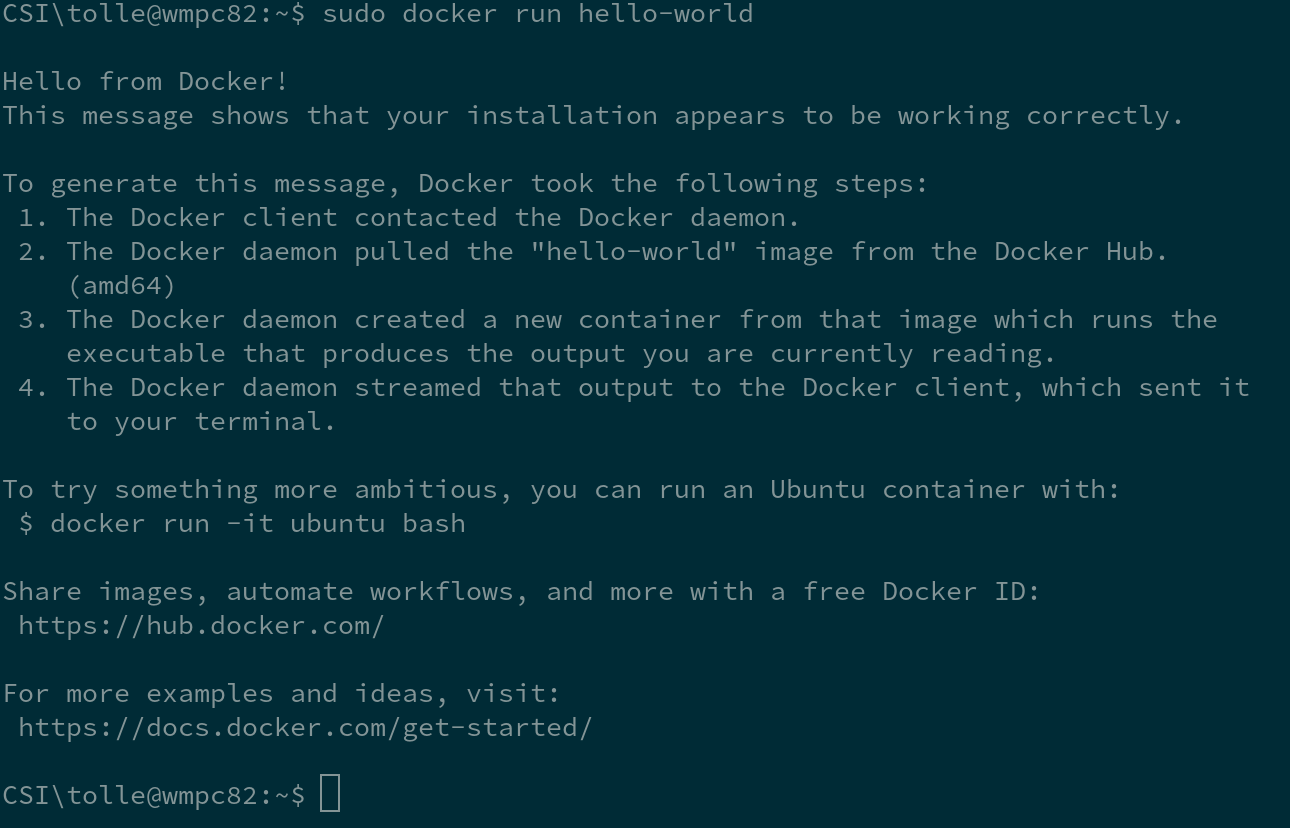
\includegraphics[width=\textwidth]{figures/docker-installation-success.png}
    \end{figure}
    \end{column}
    \end{columns}
\end{frame}
